\documentclass[12pt,letterpaper]{article}

\newenvironment{proof}{\noindent{\bf Proof:}}{\qed\bigskip}

\newtheorem{theorem}{Theorem}
\newtheorem{corollary}{Corollary}
\newtheorem{lemma}{Lemma} 
\newtheorem{claim}{Claim}
\newtheorem{fact}{Fact}
\newtheorem{definition}{Definition}
\newtheorem{assumption}{Assumption}
\newtheorem{observation}{Observation}
\newtheorem{example}{Example}
\newcommand{\qed}{\rule{7pt}{7pt}}

\newcommand{\assignment}[4]{
\thispagestyle{plain} 
\newpage
\setcounter{page}{1}
\noindent
\begin{center}
\framebox{ \vbox{ \hbox to 6.28in
{\bf CS412: ntroduction to Data Mining \hfill #1}
\vspace{4mm}
\hbox to 6.28in
{\hspace{2.5in}\large\mbox{Problem Set #2}}
\vspace{4mm}
\hbox to 6.28in
{{\it Handed Out: #3 \hfill Due: #4}}
}}
\end{center}
}

\newcommand{\solution}[4]{
\thispagestyle{plain} 
\newpage
\setcounter{page}{1}
\noindent
\begin{center}
\framebox{ \vbox{ \hbox to 6.28in
{\bf CS412:   Introduction to Data Mining \hfill #4}
\vspace{4mm}
\hbox to 6.28in
{\hspace{2.5in}\large\mbox{#3}}
\vspace{4mm}
\hbox to 6.28in
{#1 \hfill {\it #2}}
}}
\end{center}
\markright{#1}
}

\newenvironment{algorithm}
{\begin{center}
\begin{tabular}{|l|}
\hline
\begin{minipage}{1in}
\begin{tabbing}
\quad\=\qquad\=\qquad\=\qquad\=\qquad\=\qquad\=\qquad\=\kill}
{\end{tabbing}
\end{minipage} \\
\hline
\end{tabular}
\end{center}}

\def\Comment#1{\textsf{\textsl{$\langle\!\langle$#1\/$\rangle\!\rangle$}}}


%\documentclass{article}
\usepackage{amsmath}
\usepackage{algorithm}
\usepackage{algpseudocode}
\setlength{\parindent}{0pt}
\usepackage{graphicx}
\usepackage{ctable}
%\usepackage{fullpage}
%\usepackage{setspace} 
\usepackage{float}
%\usepackage{listings} 
%\usepackage{bbm}
\usepackage{bigstrut}
%\usepackage{caption}
%\usepackage{subcaption}
%\usepackage{algpseudocode}
%\usepackage{algorithm}

\usepackage{listings}
\usepackage{color}
\usepackage[utf8]{inputenc}

\definecolor{dkgreen}{rgb}{0,0.6,0}
\definecolor{gray}{rgb}{0.5,0.5,0.5}
\definecolor{mauve}{rgb}{0.58,0,0.82}

\lstset{frame=tb,
  language=matlab,
  aboveskip=3mm,
  belowskip=3mm,
  showstringspaces=false,
  columns=flexible,
  basicstyle={\small\ttfamily},
  numbers=none,
  numberstyle=\tiny\color{gray},
  keywordstyle=\color{blue},
  commentstyle=\color{dkgreen},
  stringstyle=\color{mauve},
  breaklines=true,
  breakatwhitespace=true,
  tabsize=3
}


\oddsidemargin 0in
\evensidemargin 0in
\textwidth 6.5in
\topmargin -0.5in
\textheight 9.0in
\usepackage{multirow}
\usepackage{hyperref}

\hypersetup{colorlinks=true}
\usepackage{color}

\newenvironment{ans}{%
	\vspace{5mm}
	\textcolor{red}{{\sf Answer}}\\%
}
{%
}

\begin{document}


\solution{}{Due: 12/1/2015 11:59pm}{Assignment 5}{Fall 2015}
% Fill in the above, for example, as follows:
% \solution{Joe Smith}{\today}{1}{Fall 2012}

\pagestyle{myheadings}  % Leave this command alone

\paragraph*{General Instruction}
\begin{itemize}\vspace{-2mm}\setlength\itemsep{0mm}
	\item Errata: After the assignment is released, any further corrections of errors or clarifications will be posted at \href{https://piazza.com/class/idqujg4tiae3q0?cid=93}{the Errata page at Piazza}. Please watch it.
	\item Feel free to talk to other members of the class while doing the homework. We are more concerned that
	you learn how to solve the problem than that you solve it entirely on your own. You should, however, write the solution yourself. 
	\item Please use Piazza first if you have questions about the homework. Also feel free to send us e-mails and come to office hours. 
	\item For each question, you should show the necessary calculation steps and reasoning---not only final results. Keep the solution brief and clear.
	\item For a good balance of cognitive activities, we label each question with an activity type:
	\begin{itemize}
		\item {\bf L1 (Knowledge)} Definitions, propositions, basic concepts.
		\item {\bf L2 (Practice)} Repeating and practicing algorithms/procedures.
		\item {\bf L3 (Application)} Critical thinking to apply, analyze, and assess.
	\end{itemize}
\end{itemize}
\paragraph*{Assignment Submission}
\begin{itemize}\vspace{-2mm}\setlength\itemsep{0mm}
	\setlength{\itemsep}{2pt}
	\item Please submit your work before the due time. \textbf{We do NOT accept late submission!}
	\item 
	Please submit your answers electronically via  \href{http://compass2g.illinois.edu}{Compass}. Contact CITES/TAs if you have technical difficulties in submitting the assignment.
	\item Please {\bf type} your answers in an \textbf{Answer Document}, and submit it in PDF. \textbf{Handwritten answers or hand-drawn pictures} \textbf{are not acceptable}. Your answers to all questions (including mini-MP) should be included in one Answer Document.
	\item Please \textbf{DO NOT} zip the Answer Document (PDF) so that the graders can read it directly on Compass.  
	Compress other files into a single zip file. Overall, you need to submit one Answer Document (PDF file), named as \texttt{hw5\_netid.pdf}, and one \texttt{zip} file, named as \texttt{hw5\_netid.zip}.
	\item If scripts are used, you should submit the source code, and use file names to identify the questions or sub-questions being answered. E.g., \texttt{question1\_netid.py} is the python code for Question 1; and \texttt{question1a\_netid.py} that for sub-question 1(a). You can submit separate files for sub-questions or a single file for the entire question. 
\end{itemize}
\section{Conceptual Questions (10 points)}
\begin{itemize}
\item[a.]  (L3, 2') Given the same parameters, does DBSCAN always output the same cluster assignment or not? Briefly explain.
\item[b.]  (L3, 2') With improper choice of initial cluster centers, K-Means can give us a very bad clustering output. Could you propose a method to alleviate the issue?
\item[c.]  (L1, 2') Between $k$-Medoids (PAM) and $k$-Means, which is more efficient? Briefly explain.
\item[d.]  (L1, 2') OPTICS is superior to DBSCAN because we do not have to set the paramenter $\epsilon$. True or False? Briefly explain.
\item[e.] (L1, 2') Is it true that Lazy learners (e.g., $k$NN) is more efficient than non-lazy learners (e.g., decision trees)?
\end{itemize}
\section{$k$-Nearest Neighbors (10 points)}
You will use $k$-nearest-neighbor classifier to predict labels for new data points, and investigate under what situations $k$NN works well. The set of labeled data points are given in Tabel~\ref{tab:knn}.\\

\textbf{Purpose} 
\begin{itemize}
	\item Understand how $k$NN works and its pros and cons.
\end{itemize}

\textbf{Requirements}
\begin{itemize}
	
	\item No need to use distance-weighted labels of nearest neighbors.
	\item Show your calculations for questions asking for a number.
\end{itemize}


\begin{table}[ht]
	\centering
	\begin{tabular}{l|cc|r}
		\textbf{id} & \multicolumn{1}{l}{$x$} & \multicolumn{1}{l|}{$y$} & \multicolumn{1}{l}{\textbf{label}} \\ \hline
		1           & 0                       & 0                        & +1                                 \\
		2           & 0                       & 1                        & +1                                 \\
		3           & 1                       & 0                        & -1                                 \\
		4           & 1                       & 1                        & -1                                 \\
		5           & 1.5                     & 0.5                      & +1                                 \\
		6           & 2                       & 0.5                      & -1                                
	\end{tabular}
	\caption{Data for $k$NN}
	\label{tab:knn}	
\end{table}


\begin{enumerate}
	\item[a.] (L2, 2')  Plot the given labeled data in the $x$-$y$ plane, and highlight the regions where data will be classified as `+1' by a $1$NN classifier (i.e, $k$NN for $k=1$).

	
	\item[b.] (L2, 2') Suppose we use a $3$NN classifier based on 100 (labeled) data points uniformly distributed in a {\it $d$-dimensional unit cube}, i.e.\ $[0,1]^d$. For $d=2$ (i.e, the unit square), what is the minimum size of a {\it $d$-dimensional cube centered at $q$} for it to cover at least 3 neighbors of $q$ in expectation? Show your steps. (Note that there is no need to consider the special case in which the query point $q$ lies near the boundary of the unit cube.)

	\item[c.] (L2, 2') Calculate the minimum cube size asked in (b) for $d=100$.

	\item[d.] (L3, 2') According to your calculations in (b) and (c), do you see any problem in applying a $k$NN classifier to data in high-dimensional spaces (e.g.\ $d=100$)? Briefly explain. ({\it Hint: consider the underlying principle of why $k$NN works generally.})

	
	\item[e.] (L3, 2') What are the pros and cons of using a large $k$ for the $k$NN classifier?
\end{enumerate}



%==================================================
\section{Perceptrons (12 points)}
You will design neurons and neural networks to implement some specified functions.\\

\textbf{Purpose} 
\begin{itemize}
	\item Understand how neurons and neural network approximates functions.
	\item See the different modeling capacities of perceptrons and multiple-layer neural networks (multiplayer perceptrons).
\end{itemize}

\textbf{Requirements}
\begin{itemize}	
	\item Show the neurons and neural networks using diagrams.
\end{itemize}

\begin{enumerate}
	\item[a.] (L2, 2') Given $x_1,x_2\in \{0,1\}$, design a neuron that implements the logical operation {\it AND}.  That is, the neuron takes $x_1$ and $x_2$ as input and computes $y=x_1 \text{ AND } x_2$ as output ($y\in \{0,1\}$) ({\it Hint: use the activation function $threshold(a)=1$ if $a>0$ and 0 otherwise}.)

	
	\item[b.] (L2, 2') Design a neuron that outputs $y=x_1 \text{ OR } x_2$.

	\item[c.] (L2, 2') Design a neuron that takes a single input $x\in\{0,1\}$ and outputs $y=\text{ NOT } x$.

	
	\item[d.] (L3, 4') Design a neural network that takes $x_1, x_2\in \{0,1\}$ as input and computes $y=x_1 \text{ XOR } x_2$ as output ($x_1\text{ XOR }x_2=1$ if and only if $x_1\neq x_2$). ({\it Hint: you can reuse the neurons you designed in (a)--(c)})
	
	
	\item[e.] (L3, 2') Is it possible to implement XOR using a single layer neural network (without any hidden layer)? Explain your answer.

\end{enumerate}

\section{Hierarchical Agglomerative Clustering and B-Cubed Evaluation (8 points)}
\textbf{Purpose} 
\begin{itemize}
	\item Understand how AGNES and B-Cubed work.
\end{itemize}

\textbf{Requirements}
\begin{itemize}
	
	\item In sub-question a, only draw the dendrogram.
	\item In sub-question b, only list the members of each cluster.
	\item In sub-question c, show detailed calculations of B-Cubed precision and recall.
\end{itemize}

Suppose we have 13 data points as listed and plotted in
Figure~\ref{clustering_data}. The ground truth (the correct clustering) is
also provided. 

\begin{figure}[htbp]
    \begin{minipage}[b]{.5\textwidth }
     \centering
% Table generated by Excel2LaTeX from sheet 'Sheet2'

    \begin{tabular}{|c|c|c|c|}
    \hline
    Point    & x    & y & 
    Ground-truth cluster \bigstrut\\
    \hline
    P1     & 1   & 3 & C1 \bigstrut\\
    \hline
    P2     & 1   & 2 & C1 \bigstrut\\
    \hline
    P3   & 2   & 1 & C1\bigstrut\\
    \hline
    P4     & 2   & 2 & C1\bigstrut\\
    \hline
    P5   & 2     & 3 & C1\bigstrut\\
    \hline
    P6   & 3     & 2 & C1\bigstrut\\
    \hline
    P7   & 4   & 3 & C1\bigstrut\\
    \hline
    P8   & 6     & 3 & C2\bigstrut\\
    \hline
    P9   & 4     & 5 & C2\bigstrut\\
    \hline
    P10   & 5     & 4 & C2\bigstrut\\
    \hline
    P11   & 5     & 5 & C2\bigstrut\\
    \hline
    P12   & 6     & 4 & C2\bigstrut\\
    \hline
    P13   & 6     & 5 & C2\bigstrut\\
    \hline
    \end{tabular}%
 %       \caption{Training data}
        %\label{thelabeltab}
        \vspace{0pt}
    \end{minipage}%
    \begin{minipage}[b]{.5\textwidth}
   \centering
        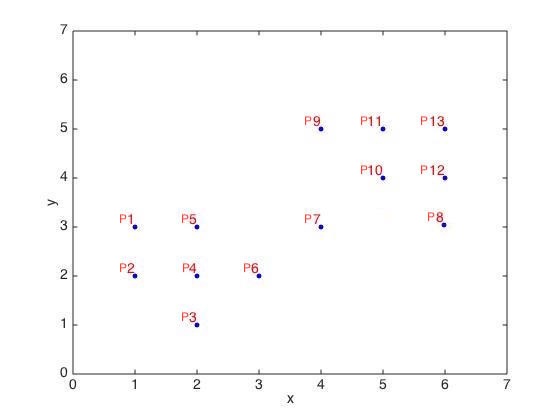
\includegraphics[width=\textwidth]{fig/clustering_data.jpg}
     \centering
        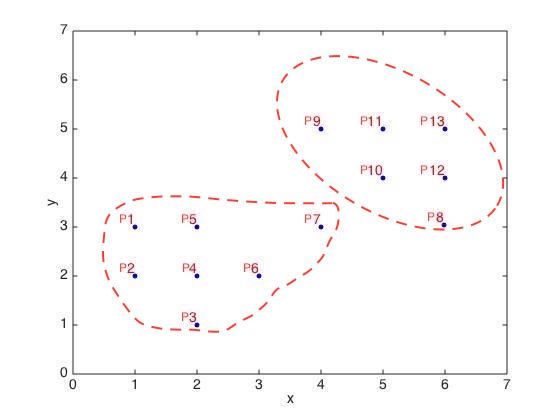
\includegraphics[width=\textwidth]{fig/clustering_truth.jpg}
    \end{minipage}
    \caption{Data and ground truth}
    \label{clustering_data}
\end{figure}

\begin{itemize}
\item[a.]  (L2, 4') Draw the dendrogram using AGNES. Please use {\it single link} and {\it Euclidean
distance} as the dissimilarity measure.

\item[b.]  (L2, 2') If we want to cluster
the dataset into 3 groups based on the dendrogram, what are the members of each of the 3 groups? 

\item[c.]  (L2, 2')  Based on the given ground
truth, what are the {\it B-Cubed} precision and recall of the
output? 
\end{itemize}

\section {K-Means (8 points)}

\textbf{Purpose} 
\begin{itemize}
	\item Understand how $k$-Means works.
\end{itemize}

\textbf{Requirements}
\begin{itemize}
	\item In sub-question a and b, for each iteration of $k$-Means:
	\begin{itemize}
	    \item Annotate the data points in figure~\ref{clustering_data} to show which points belong to which clusters, e.g., draw a red circle at each point belonging to cluster 1, and green and blue circles for cluster 2 and cluster 3. (The file for the figure is provided in {\tt data.zip}.)
        \item Plot the mean of each cluster with the same color you use for data points in this cluster, but in different shape to differentiate them from data points.
        \item Show the coordinates of the cluster centers in each iteration.
        \item Do not include scanned pictures. You might use annotation or image processing tools such
as Mac Preview or Microsoft Paint to annotate the file.
        \item Do not show numerical distances in each iteration.
	\end{itemize}
	\item In sub-question c, any reasonable method with brief explanation is acceptable.
\end{itemize}

We will use the same data as question 4 (figure~\ref{clustering_data}).

\begin{itemize}
\item[a.]  (L2, 4') Perform $k$-means using Euclidean distance with $k=2$ and the initial cluster
centers $P1$ and $P2$. 

\item[b.]  (L2, 2') Perform $k$-means using Euclidean distance with $k=2$ and the initial cluster
centers $P2$ and $P12$. 
\item[c.]  (L3, 2') As you can see in sub-questions a and b, choices of initial cluster centers can affect the speed of the clustering process. Assume $k=2$ and the data are 2-dimensional, suggest a general and reasonable way to select initial cluster centers to speed up the clustering process. Briefly justify your choice.  
\end{itemize}

\section{Machine Problem (50 points)}

\textbf{Purposes}
\begin{itemize}
\item Get deeper understanding and working experience of DBSCAN algorithm and B-Cubed evaluation through implementation and result visualization.
\item Get hands-on experience with cluster analysis using Weka.
\end{itemize}

\textbf{General Requirements}
\begin{itemize}
\item This is the second and the last MP (not a mini one) we have in this course. It consists of several programming tasks, which usually take more time than written assignments, so please \textcolor{red}{start early}.
\item This is an \textcolor{red}{individual assignment}, which means it is OK to discuss with your classmates and TAs regarding the methods, but it is \textcolor{red}{not OK} to work together or share code.
\item Libraries or programs of cluster analysis algorithms can be found on-line, but \textcolor{red}{you are prohibited} from using these resources directly. This means you can not include external libraries, or modify existing programs, since the purpose of this MP is to help you go through DBSCAN step by step.
\item You can use Java/C++/Python as your programming language. No other languages are allowed.
\item Each sub question will contain detailed requirements. Please note that most of them require you to not only submit code but also write discussions, report results, or draw graphs. If you submit code without answering those questions, you will receive 0 point.
\item Put all your codes in a separate folder with the name {\tt NetId\_assign5\_codes}. Do not use sub-folders inside this folder. All of your codes should have been successfully compiled before submission. Do not include files other than the codes you write. Put a single {\tt readme.txt} file in the code folder to briefly describe your codes and how to run them.
\item Put the results you generate in another folder with the name {\tt NetId\_assign5\_results}. 
\item Compress folder {\tt NetId\_assign5\_codes} and {\tt NetId\_assign5\_results} into a single zip file, and name it {\tt NetId\_assign5.zip}. Submit both this zip file and Answer Document {\tt NetId\_assign5\_answer.pdf} through Compass2g. \textcolor{red}{Please do not zip the PDF file!} 
\item If you copy source code from other students or external sources, you will receive a serious penalty. We will run plagiarism detection
software. Please do not cheat.
\end{itemize}

\textbf{Description of Data}
\begin{itemize}
\item You can find {\tt data-hw5.zip} from \href{https://wiki.cites.illinois.edu/wiki/display/cs412fa15/Assignments}{the course website}. It contains three files: {\tt data.txt}, {\tt data.arff}, and {\tt truth.txt}.
\item The description of {\tt data.txt} is as follows:
\begin{itemize}
\item The first line contains an integer $n$ as the number of data points.
\item Each of the $n$ following lines corresponds to a 2-dimensional data point, which contains two floating-point numbers as the coordinates of a point. They are separated by a comma.


\end{itemize}
\item File {\tt data.arff} is a Weka-friendly version of {\tt data.txt}. 
\item File {\tt truth.txt} is the ground truth of clustering for the data in {\tt data.txt}. It is hand-labeled by domain experts. The description of {\tt truth.txt} is as follows:
\begin{itemize}
\item The first line contains an integer $n$ as the number of data points.
\item The second line contains an integer $m$ as the number of clusters.
\item Each of the $n$ following lines corresponds to a 2-dimensional data point in {\tt data.txt}, which contains three numbers, where the first two are the coordinates of the point, and the last one is an integer $c \in \{1 \ldots m\}$ indicating the point belongs to cluster $c$, and $c=0$ if the point is an outlier. The three numbers are separated by commas. Please note that the name/index of each cluster is unimportant. It is just a notation to indicate which points belong to the same cluster.
\end{itemize}
\end{itemize}

\begin{enumerate}
\item[Step 0:] $(0')$ \textbf{Normalizing Data.}

The first step you need to do is preprocessing data. In this assignment, you should min-max normalize each dimension of the data. The formula is as follows:
$$x\_normalized=\frac{x-minX}{maxX-minX}$$

We also provide you with the min-max-normalized data in file {\tt data-normalized-hw5.zip} from \href{https://wiki.cites.illinois.edu/wiki/display/cs412fa15/Assignments}{the course website}.

\item[Step 1:] $(23', L3)$ \textbf{Implementing DBSCAN.} 
  
In this step, you need to implement DBSCAN: 
\begin{itemize}
\item Name: {\tt dbscan.java}, or {\tt dbscan.py}, or {\tt dbscan.cpp}
\item Input
\begin{itemize}
\item Dataset file, e.g., {\tt /home/mike/mike\_assign5/mike\_assign5\_data/data.txt}
\item Output file, e.g., {\tt /home/mike/mike\_assign5/mike\_assign5\_results/step1.txt}
\item Parameter $MinPts$, e.g, 25
\item Parameter $\epsilon$, e.g, 0.065
\end{itemize}
\item The structure of output file:
\begin{itemize}
\item The first line contains $minPts$ 
\item The second line contains $\epsilon$
\item The third line contains the number of clusters
\item Each of the $n$ following lines corresponds to a 2-dimensional data point in {\tt data.txt}, which contains three numbers, where the first two are the coordinates of the point, and the last one is integer $c \in \{1 \ldots m\}$ if the point belongs to cluster $c$, or $c=0$ if the point is an outlier. The three numbers are separated by comma characters.
\end{itemize}
\end{itemize}

As it is hard for humans to interpret the output, you need to visualize it. In particular, do a scatterplot for all the data points, and color the points according to the clustering. For example, all outlier points are black, all the points belonging to cluster 1 are red, all the points belonging to cluster 2 are blue, etc. You can create the plot using MATLAB, Excel or any tools you like. You do not need to include the code for creating the graph.

\textbf{Requirements:}
\begin{itemize}
\item Put your DBSCAN source code to folder {\tt NetId\_assign5\_codes}
\item Run your program on the given data file with $MinPts=25$ and $\epsilon=0.065$ so that we can check the correctness of your code by looking at the output file. Name the output file as {\tt step1.txt}, and put it to folder {\tt NetId\_assign5\_results}.
\item Include in your Answer Document two scatterplots, one for your output and one for the ground truth.
\item \textit{Question to ponder A: How long does it take for your machine to run DBSCAN on the given data? What is the time complexity of DBSCAN in the worst case scenario? Can you describe a worst case scenario?}
\item \textit{Question to ponder B: Usually, a good clustering algorithm should put similar points to the same cluster, and dissimilar points to different clusters. Based on that intuition, what do you think of the clustering result? Given the same $MinPts$, should we increase or decrease $\epsilon$ to get more intuitive clustering results?}
\end{itemize}
  
\item[Step 2:] $(10', L3)$ \textbf{Parameter tuning for DBSCAN.}

Given $MinPts=25$, find two new $\epsilon$ such that the numbers of clusters in the corresponding results are different from each other and from the $\epsilon$ in step 1. 

\textbf{Requirements:}
\begin{itemize}
\item Run DBSCAN two times with the two $\epsilon$ described above, and create two output files with the format similar to {\tt step1.txt}. Name them as {\tt step2a.txt} and {\tt step2b.txt}, and put them to folder {\tt NetId\_assign3\_results}
\item Create a table in the answer document to report the number of clusters, and the number of outliers corresponding to each of the two new $\epsilon$ and the $\epsilon$ in step 1 (your table should have three rows excluding the header).
\item Draw two scatter plots corresponding to the two new $\epsilon$. Include them in the Answer Document.
\item \textit{Question to ponder C: Which one of three $\epsilon$ is the best? Could you suggest a general way to tune parameters $MinPts$ and $\epsilon$ for DBSCAN?}
\end{itemize}

\item[Step 3:] $(7', L3)$  \textbf{Implementing B-Cubed evaluation.}

In this step, you need to implement B-Cubed evaluation:
\begin{itemize}
\item Name: {\tt bcubed.java}, or {\tt bcubed.py}, or {\tt bcubed.cpp}
\item Input: two parameters:
\begin{itemize}
\item Clustering output file, e.g., {\tt /home/mike/mike\_assign5/mike\_assign5\_results/step1.txt}
\item Ground truth file, e.g., {\tt /home/mike/mike\_assign5/mike\_assign5\_data/truth.txt}
\end{itemize}
\item Output: Two lines in {\tt stdout}
\begin{itemize}
\item The first line contains {\it precision}
\item The second line contains {\it recall}
\end{itemize}
\end{itemize}

\textbf{Requirements:}
\begin{itemize}
\item Put your B-Cubed source code to folder {\tt NetId\_assign5\_codes}
\item Run B-Cubed with the outputs from Step 1 and Step 2. Create a table to report the {\it precision} and {\it recall} corresponding to each of the outputs.
\item \textit{Question to ponder D: Can you suggest a way to combine B-Cubed precision and recall into a single measure so that it would be easier to compare different results?}
\end{itemize}
 
\item[Step 4:] $(10', L2)$  \textbf{Doing cluster analysis by Weka.} 

In class, we have demonstrated how to do this. You can watch the online lecture video to review the process. We also provide the procedure below.

    \begin{enumerate}
	\item Open Weka.
    \item Choose \texttt{Explorer}.
    \item Click on \texttt{Preprocess} tag.
    \item Click on \texttt{Open file}, choose {\tt data.arff} , click on \texttt{Choose} and wait until Weka finishes loading the data.
    \item Click on \texttt{Cluster} tag. Here you can find common algorithms for cluster analysis, such as OPTICS, DBSCAN, etc.
    \end{enumerate}

\textbf{Requirements:}
\begin{itemize}
\item Run {\tt SimpleKMeans} with different number of clusters. Report the best number of clusters, and the plot showing the corresponding clustering result. You can generate the plot by right clicking on the entry of the {\tt Result list}, and choose {\tt Visualize cluster assignments}.
    \item Run DBSCAN with the best $minPts$ and $\epsilon$ in Step 2. Show the plot for the corresponding clustering result.
\item \textit{Question to ponder E: Compare the results from $k$-Means and DBSCAN. Is $k$-Means or DBSCAN more suitable for the provided dataset? Why?}
\end{itemize}

\end{enumerate}
\end{document}